
\chapter{Data Management on an Industrial Scale}
\label{ch01}

In our modern economy, the finance industry arguably drives all other industries. No matter whether a company is repeating a tried and true business formula, or if it is innovating and creating new markets, it needs to manage capital; make investments, take loans, manage cash flows.  The finance industry has developed a vast array of products and services to support business in all its various forms.  This variety provides flexibility to support businesses in every stage of development, from small family businesses to international conglomerates.  But as a result, the finance industry is notoriously complex and prone to corruption and abuse. It seems that just about every day one can find a story in a newspaper about some violation of trust committed by a financial institution somewhere in the world. Because of its complexity, the financial industry seems opaque and incomprehensible, even to sophisticated practitioners in many  fields. To deal with this lack of trust, the finance industry has become one of the most highly regulated industries in today’s world.  But regulations only sweep the problem under the rug; the real issue is that no single person or entity really understands the whole finance system; it really does behave as if it has a mind of its own. 

There are many paths we can take toward improving this situation, and we will probably have to progress along all of them.  This book follows a path set out in 2013 with the publication by the Based Commission on Banking Supervision of the Principles for effective risk data aggregation \cite{basel2013principles}, known as BCBS239 for short. One of the basic tenets of BCBS 239 is that consistent management of data in the finance industry is essential for understanding the complexities of financial instruments and services.  

In this book, we describe the Finance Industry Business Ontology (FIBO), which responds to the need identified in BCBS239.  FIBO is an ontology written in the Web Ontology Language (OWL), and, as such, describes the structure of data about entities in the finance industry.  FIBO has quite a broad scope, and covers business entities, commerce, loans, securities (including derivatives), and indices.  

FIBO is an ontology; details of what this means for FIBO can be found in \cite{KendallMcGuinness 2019} and \cite{AllemangHendler2020}.  For the purposes of our work here, there are  three aspects of an ontology that are important:
\begin{enumerate}
    \item FIBO is {\it referenceable}; that is, data models and data sets can refer to elements in FIBO.  FIBO is written in the Semantic Web language OWL, so these references are to URIs for the entities in FIBO. 
    \item FIBO describes data; FIBO is not itself a data source, but a resource to describe data about instruments, services, entities, etc. 
    \item FIBO is based on logic; this means that it is composed of a collection of statements in logic.  It is possible to treat these statements as you would any set of logical axiom; draw inferences from them, or determine if they are consistent.
\end{enumerate}

It is important to understand as well what FIBO is not.  
\begin{enumerate}
    \item FIBO is not a database.  While it is possible to query FIBO, it has no information about any particular instrument, entity or service. 
    \item FIBO is not a data schema.  It is not expected that it will be used to create a database to match the entities in FIBO. 
\end{enumerate}

\section{Using FIBO}

Since FIBO is a reference model that describes data, but not itself a database or a schema, how can someone use FIBO?  We will examine detailed use cases in later chapters, but in this section we will outline the mechanics of some of the ways data managers typically use FIBO to help understand their data.

We'll use the following example to elaborate these uses. 

FIBO defines something called a {\it Legal Entity}; it is defined as ``legal person that is a partnership, corporation, or other organization having the capacity to negotiate contracts, assume financial obligations, and pay off debts, organized under the laws of some jurisdiction''. FIBO has a lot to say about Legal Entity, including how it is registered and organized, various ways to classify a Legal Entity, different kinds of Legal Entities, etc.  Among the things we know about a Legal Entity is that it has two different addresses; a {\it headquarters address} and a {\it legal address}. Each of these things is an address, which has four parts (among others): a {\it street address},  a {\it city name}, {\it subdivision (e.g., state)}, and {\it postal code}.  

We can use this fragment of FIBO in the following ways: 

\begin{enumerate}
    \item As a starter model for a data schema.  If we want to represent a legal entity in a data system, we can consult FIBO for advice.  In this example, FIBO will suggest that we provide two, not just one, addresses for the legal entity.  We might not have been aware of the distinction between legal address and headquarters address beforehand. 
    \item As a validation of data models we find in our applications.  If we have a table in a database about a legal entity, and it has fields with names like \say{ADDR1}, \say{CITY}, and \say{STATE}, we can guess that these form an address.  The reference model also includes \say{ZIP}, which might be missing in our data table.  We can't add extra fields into a functioning database, but we can note that the address is missing a field that is used by the post office.  We can also note that there is an address missing, and then ask whether the address we have is a headquarters address or a legal address. 
    \item As an explanation of existing data structures. Suppose again that we have a table in a database, but this time we find eight fields; \say{ADDR}, \say{CITY}, \say{STATE}, \say{ZIP}, \say{HQADDR}, \say{HQCITY}, \say{HQSTATE} and \say{HQZIP}.  The reference model provides an explanation of all of these; the first four and the last four each constitute an address.  The first four are the legal address, and the last four are the HQ address. 
\end{enumerate}

Each of these uses of FIBO has its strengths and weaknesses. 

\subsection{FIBO as a starter model}
Using FIBO as a starter model is probably the most obvious way to use it.  It seems natural, since data modeling is a specialized and detailed task, having a resource to make it less error prone and more predictable seems like a good idea.  And indeed, as we have already seen, a reference model like FIBO can inform a data modeler of patterns that they might not have been aware of, such as the two different kinds of addresses that a legal entity can have.  In this example, FIBO has also provided advice about structuring data; a data modeling might be considering whether the address fields should be part of a separate entity (an \say{ADDRESS}), or simply parts of the main record for the legal entity; FIBO clearly suggests the former (see \ref{ch01.fig1}).   In this way, FIBO can provide assistance to a data modeler.

\begin{figure}[hbt] % 01
\centering
  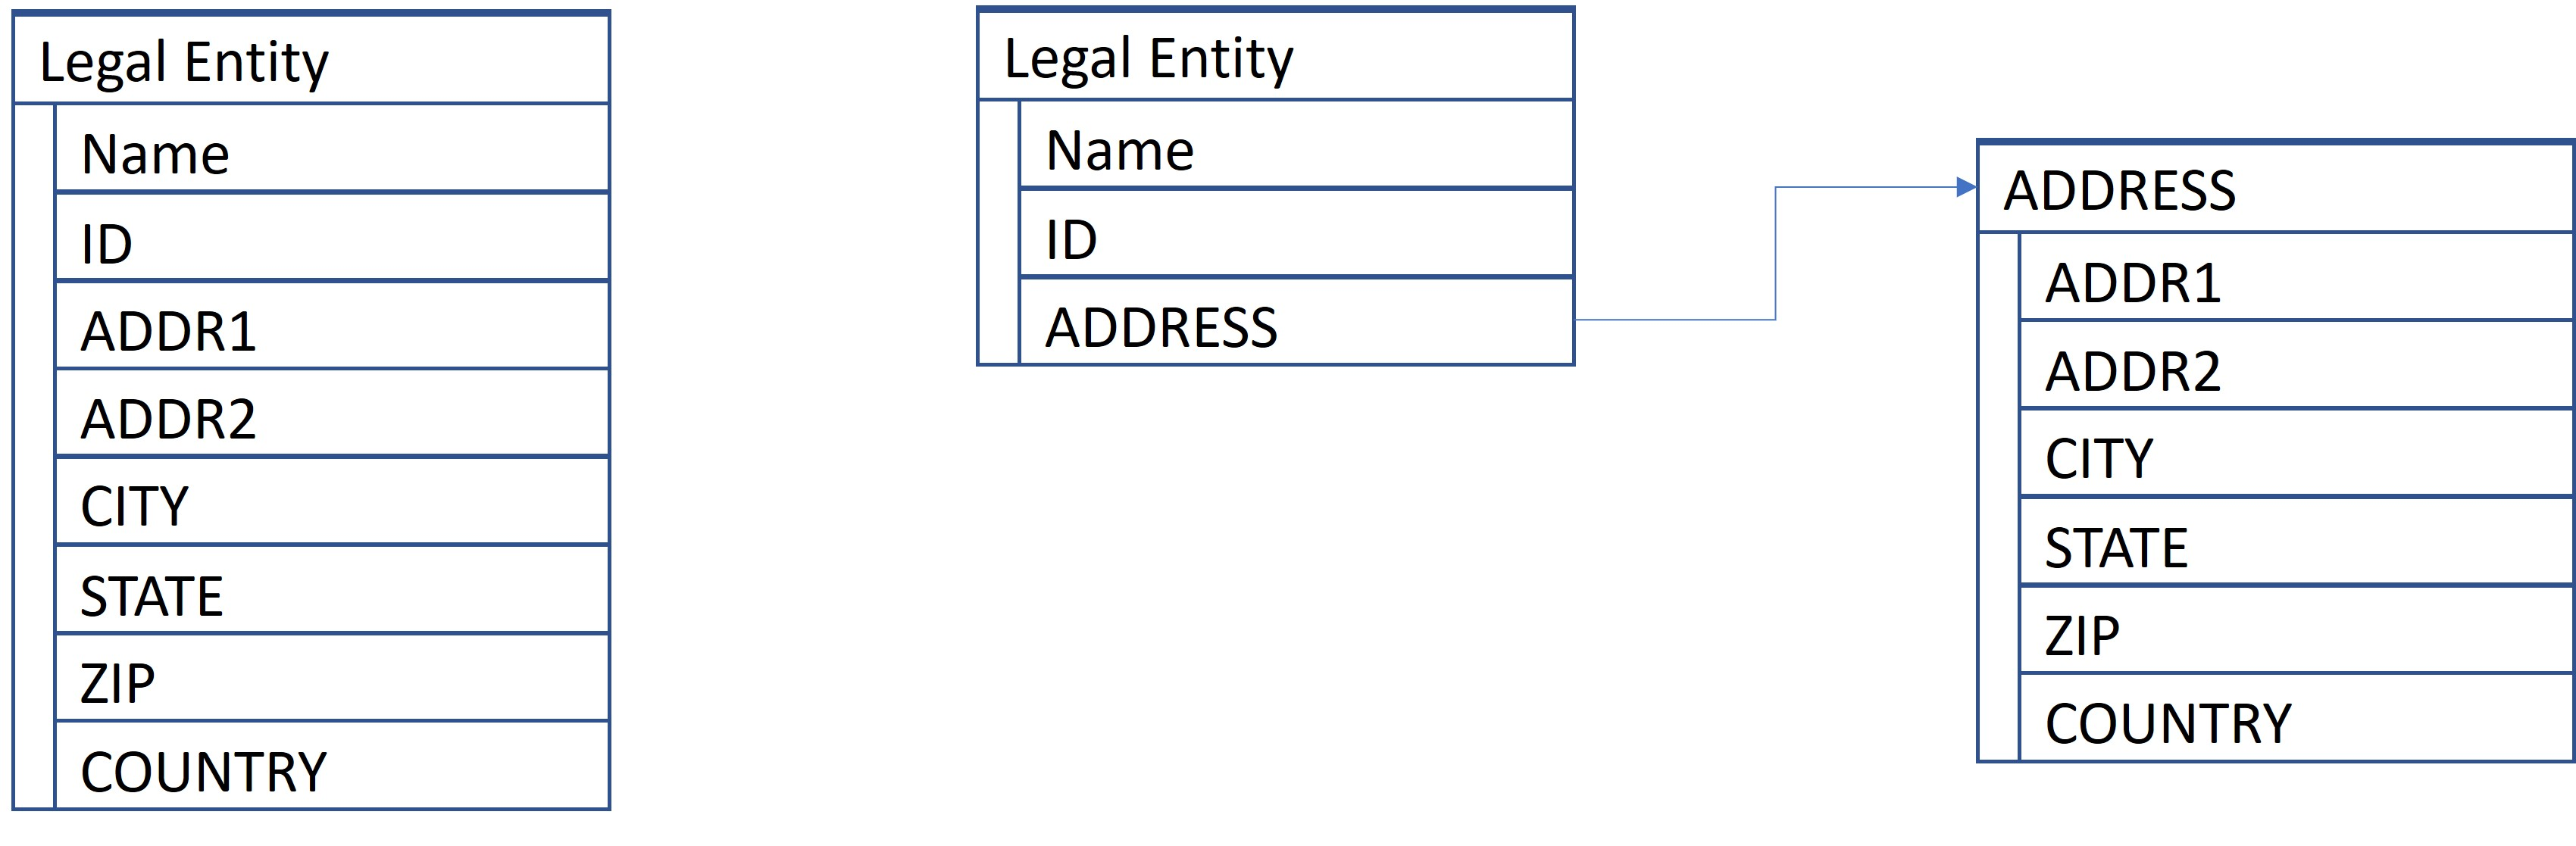
\includegraphics[width=3.3in]{figures/data-structure.jpg}
\caption{Alternate data structure; is ADDRESS its own thing, or just part of the description of a Legal Entity? }
\label{ch01.fig1} 
\end{figure}


But using a reference model like FIBO in this way can create issues as well as solve them.  In this example, a particular application might not need to track both the legal and headquarters address (e.g., it is an application that tracks the jurisdictional requirements that regulate the entity's business; the location of the headquarters is irrelevant, but the legal address is not).   The advice given by an industry model like FIBO will be, strictly speaking, 'correct', but it won't be useful or applicable in this particular situation.  In such a case, using FIBO to guide a data model will be distracting or confusing. 

If FIBO is to be used to inform a data model, the best approach is to use it as a reference guide, while building the data model.  For any property or class in FIBO, ask whether the distinction it is making is relevant to the data model in question.  FIBO is then a source of information about alternatives that might not have been considered (e.g., types of addresses) and of structure (the main reason to call out addresses as entities in their own right, is because there are potentially multiple types of them).  The final decision for the data model has to be driven by its own application needs; FIBO can provide context and alternatives. 

\subsection{FIBO as Validation Framework}

In many situations, a data model is already complete and has been in use for years in a particular application.  In such a situation, there is no benefit to be had by using FIBO as a source of design inspiration; the time for design is long past.  But the model might well have issues that can be surfaced by comparing it to a reference model like FIBO. 

In our address example, we can find missing fields such as postcode (or, perhaps more realistically, country code, for international addresses).  But the validation that FIBO provides can be more subtle and more useful.  In this example, FIBO identifies two different kinds of addresses.  Imagine that we have a running system whose data model only has one address.  But in contrast to an earlier example, the application is not tied just to legal issues; it is also used for deliveries, billing and other purposes.  How can a single address satisfy these different uses? 

It is not uncommon to find data models that have been running \say{successfully} for years to have deep data quality issues, that are compensated for in application code, workflow, or sometime just institutional knowledge (\say{Everyone knows you don't go to that system to get shipping information}).  A reference model like FIBO can shed light on situations like this, and even suggest what would need to change to fix them (in this case, determine which address is actually being stored, and notate that.  in the case where both addresses are being stored haphazardly in the same fields, a data quality overhaul may be called for). 

\subsection{FIBO for Explanation}

As a follow-on to FIBO for validation, FIBO can be used to explain and document existing data structures.  As in the previous example, suppose we have an existing data structure that is currently working in one or more applications.  But the design of the data structure was done long ago, and the individuals who worked on it have retired or move on to other posts.  The enterprise has lost an understanding of the data; it no longer knows what it knows. 

To take a more concrete example, consider the table that has eight fields as listed above, \say{ADDR}, \say{CITY}, \say{STATE}, \say{ZIP}, \say{HQADDR}, \say{HQCITY}, \say{HQSTATE} and \say{HQZIP}.  FIBO as validator could suggest a \say{COUNTRY} field for each of these, but for this discussion we want to understand how FIBO can explain these eight fields.  

\begin{figure}[hbt] % 01
\centering
  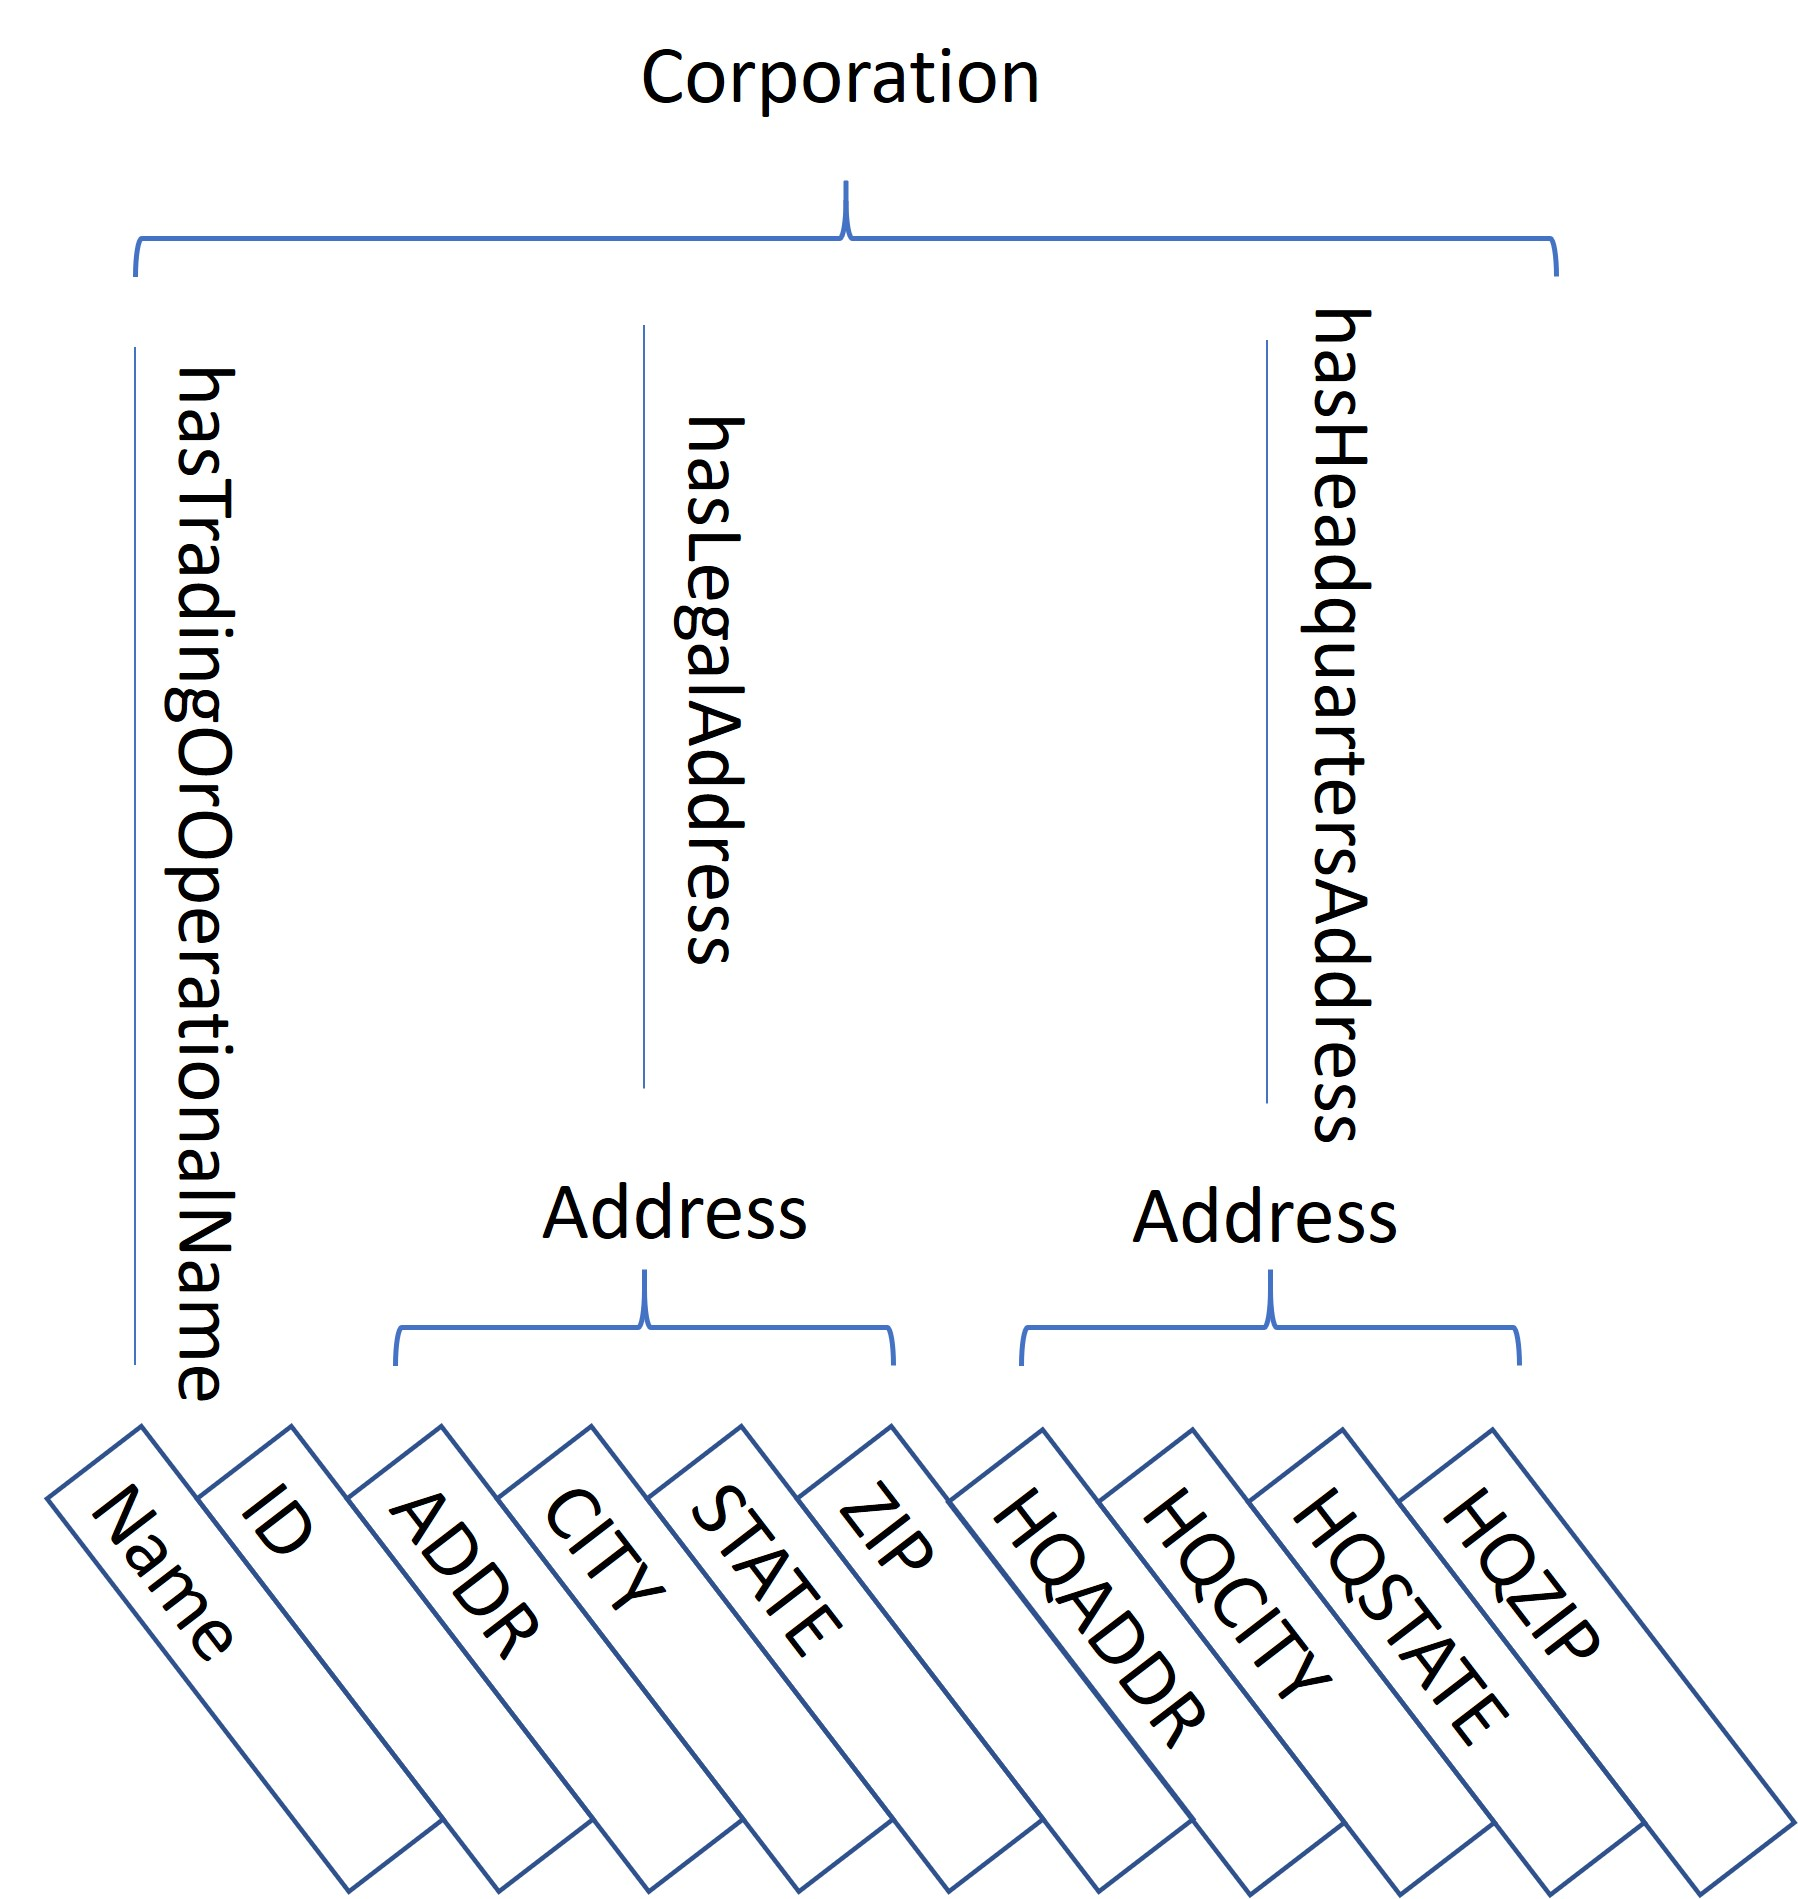
\includegraphics[width=3.3in]{figures/data-table.jpg}
\caption{FIBO providing structure for a flat database table }
\label{ch01.fig2} 
\end{figure}


Figure \ref{ch01.fig2} shows how FIBO can group the fields in the data table to explain them.  The two sets of four fields that make up an address are grouped and labelled as "Address" (which is a word from FIBO).  The symmetry among these fields is explained by the fact that they represent two occurrences of the same structure. 

Furthermore, the distinction between the two is also evident; one of them represents the headquarters address and the other the legal address.  But even in this distinction, there is something common; they represent the legal and headquarters address of the same legal entity, which is given elsewhere in the table.  This structure not only documents the meaning of the fields in the table, it relates them to a standard of meaning, allowing them to be cross-referenced with other FIBO aligned tables. 

As an example of a use case that can take advantage of this sort of machine-readable documentation, imagine a regulator who stipulates that the legal address of a legal entity is public information (since that is part of any corporate filings that they have), but that the headquarters address can be private (as is the case of sole proprietorship, where the \say{headquarters address} is often the home address of the sole proprietor themselves).  Furthermore, suppose that new privacy legislation requires that a financial institution be able to locate all private address information.   The explanation structure in Figure \ref{ch01.fig2} makes it clear which fields hold this kind of information. 

\section{Design Rationale}

Design rationale refers to the reasons why a design is the way it is; why are some components present and others absent, why are the components that are present related to one another the way they are.  For a complex field like finance, there are a wide variety of choices available for how an ontology can be built.  Why did the FIBO designers choose one solution instead of another? 

Design often involves a trade-off between competing goals.  Some common trade-offs that apply to many design problems include efficiency vs. clarity, time vs. space, and cost vs. quality.  The design of FIBO is no different; design decisions in FIBO have been made considering trade-offs between comprehensive coverage, clarity, consistency, along with many other considerations.   Since any design decision is a trade-off, there will be issues with the result; things that it should do but it does not.  Much of the discussion in this chapter will set the stage for the design trade-offs that FIBO navigates.


\section{Application, Enterprise and Industrial Data}
\label{ch01.sec1}

When we think about a data-driven application, we usually think about the data that some user interacts with through an application.  It might be an order for a product, or a standing for an account, or a position in a game.  For more niche users like analysts and developers, the data has to do with some process whose future we want to predict.  We decide what data to display, and how to present it, based on the needs of the application user. 

When we are managing data in an enterprise, we have to take a broader view.  Enterprise data isn't store just to power a single application, but a set of applications throughout the workflow of the business.  Enterprise data has to serve many masters; not only does it have to power the applications that users (including customers as well as our own employees) see, but also applications that help us run the company; risk management applications, regulatory reporting, market analysis, etc.  In order for an enterprise to run smoothly, the data from all of these applications has to form a coherent story.  Enterprise Data Management has to take into account the variety of possibilities of data usage from throughout the enterprise. 

FIBO goes one level beyond enterprise data, to what we call industrial data.  Within a single enterprise, data is used in service of the company's corporate goals; satisfying customers, providing a service or making a product.  But data is also shared between enterprises in an industry.  Regulatory data is a clear example of this sort of data; regulators need to be able to collect data from a number of different companies, and be able to understand what it means.  Market analysts have to be able to do the same thing; information about sales, utilization, supply and demand will come from multiple sources.  Industrial data management has to take into account the variety of possibilities of data usage from multiple enterprises. 

When we build an enterprise data model, we have to anticipate what sorts of data structures and distinctions will be necessary for a variety of applications.  When we build an industrial data model, we have to anticipate what sorts of data structures and distinctions will be necessary for a variety of businesses.  This kind of modeling is essentially very different from application data modeling, where we have a set of requirements for the application that we have to conform to.  When we model for the enterprise, and even more so for the industry, we have to anticipate what models we will find, in the applications in the enterprise.  A typical large enterprise has thousands of applications; in an industry, we have thousands of companies.  We can't examine all of them before we begin to build a model.  This means that our model is in the business of anticipating what sorts of data distinctions might be used in some application that we haven't seen yet.  Designing an industry-level data model involves prediction much more than building an application data model. 

For this reason, a lot of the design rationale for an industrial model like FIBO is in response to anticipated data models that it could apply to.  The role of a model like FIBO is to provide a consistent framework that provides insight into data models we haven't yet seen.


\section{Example}

As an example of the different design trade-offs of application, enterprise and industrial data, let's consider a simple example: an identifier for a legal entity. Many companies have good reason to keep track of other legal entities.  These might be customers (where the legal entities can be corporations or individuals), or competitors, or, in the case of an investment bank, the legal entities that are involved in the financial instruments that the bank writes.  

Many banks are also stockbrokers; suppose the bank wants to provide a mobile app for its investors to track the stocks in their portfolio.  The stocks of course represent equity in various legal entities.  It is customary to represent those entities, in the case of stocks, with their SEC symbols; usually a 3- to 4-letter mnemonic that indicates what company the stock is in.  The application level data needs a field that identifies the stock; this field can be a short character field that holds this symbol.  Nothing more elaborate is needed, nor appropriate.  The app works fine representing the identifier for the stock directly as a string. 

At the enterprise level, the situation is more complex.  That same legal entity has a credit rating given by various agencies (Reuters, Fitch, etc.).  It is also involved in AML/KYC data, which include the legal hierarchy (various companies that are owned by a conglomerate holding company).  Each of these systems has an identifier for the legal entity; since the bank itself is a conglomerate formed by the merger of several banks and brokerage firms, each of them had its own way of tracking these entities.  The enterprise architecture of the bank will include multiple identifiers, inherited from the data systems from the original banks.  There are a number of ways to do this; one way (and probably the most common), as shown in Figure \ref{ch01.fig3}, is to have a set of fields, one  for each identifier.  A legal entity would have a field for the SEC, the TIN, EIN, LEI, and separate fields for the bespoke identifiers that the company uses that aren't shared outside the firm.  In one example, there were over a hundred distinct identifiers that were used to identify a legal entity!  

\begin{figure}[hbt] % 01
\centering
  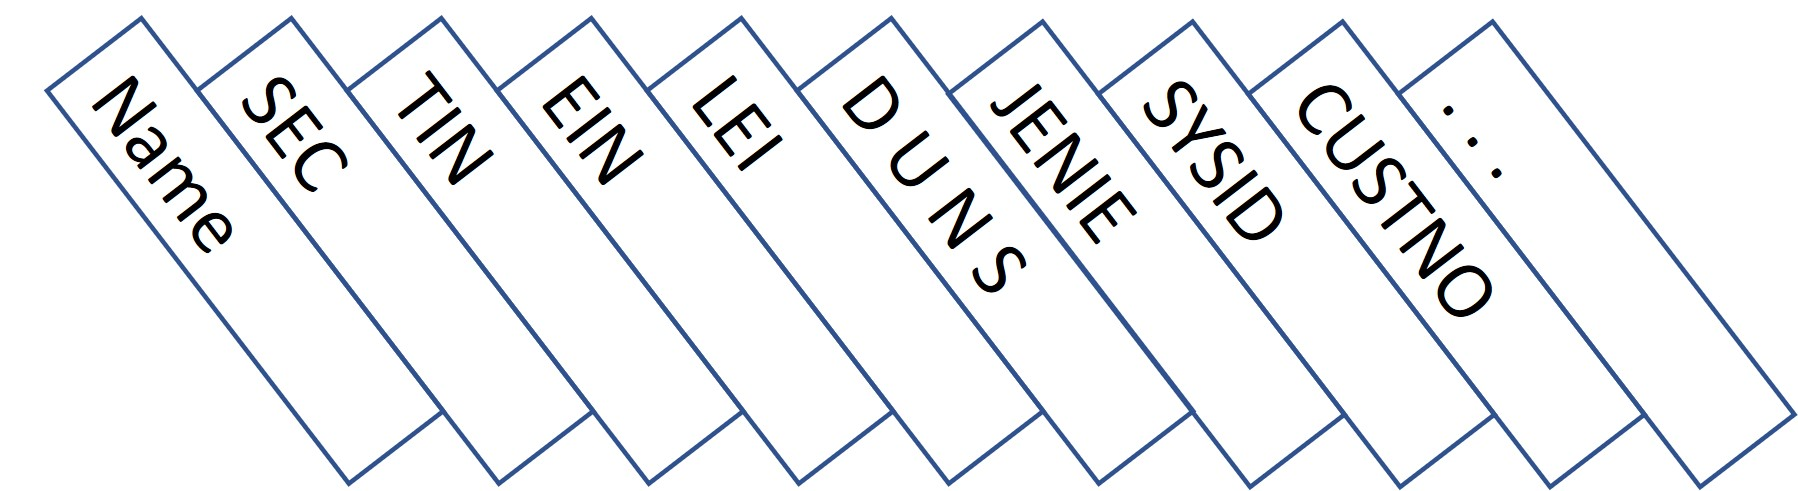
\includegraphics[width=3.3in]{figures/id-table.jpg}
\caption{Representing identifiers as character fields.  Some fields are standard IDs (SEC, TIN, EIN, LEI and DUNS), others are particular to this enterprise data system (JENIE, SYSID, CUSTNO) }
\label{ch01.fig3} 
\end{figure}

Another way to represent this, as shown in Figure \ref{ch01.fig4} is to have a separate entity for the identifier;  the identifier would have a type (SEC, EIN, TIN, LEI, etc.), and a value (probably a string).  It would also point to the entity that it identifies; in this way, any number of identifiers for a legal entity are possible.  Even in enterprise systems with a hundred identifiers, this isn't a common way to represent identifiers for legal entities; it doesn't lend itself well to supporting application code.  

\begin{figure}[hbt] % 01
\centering
  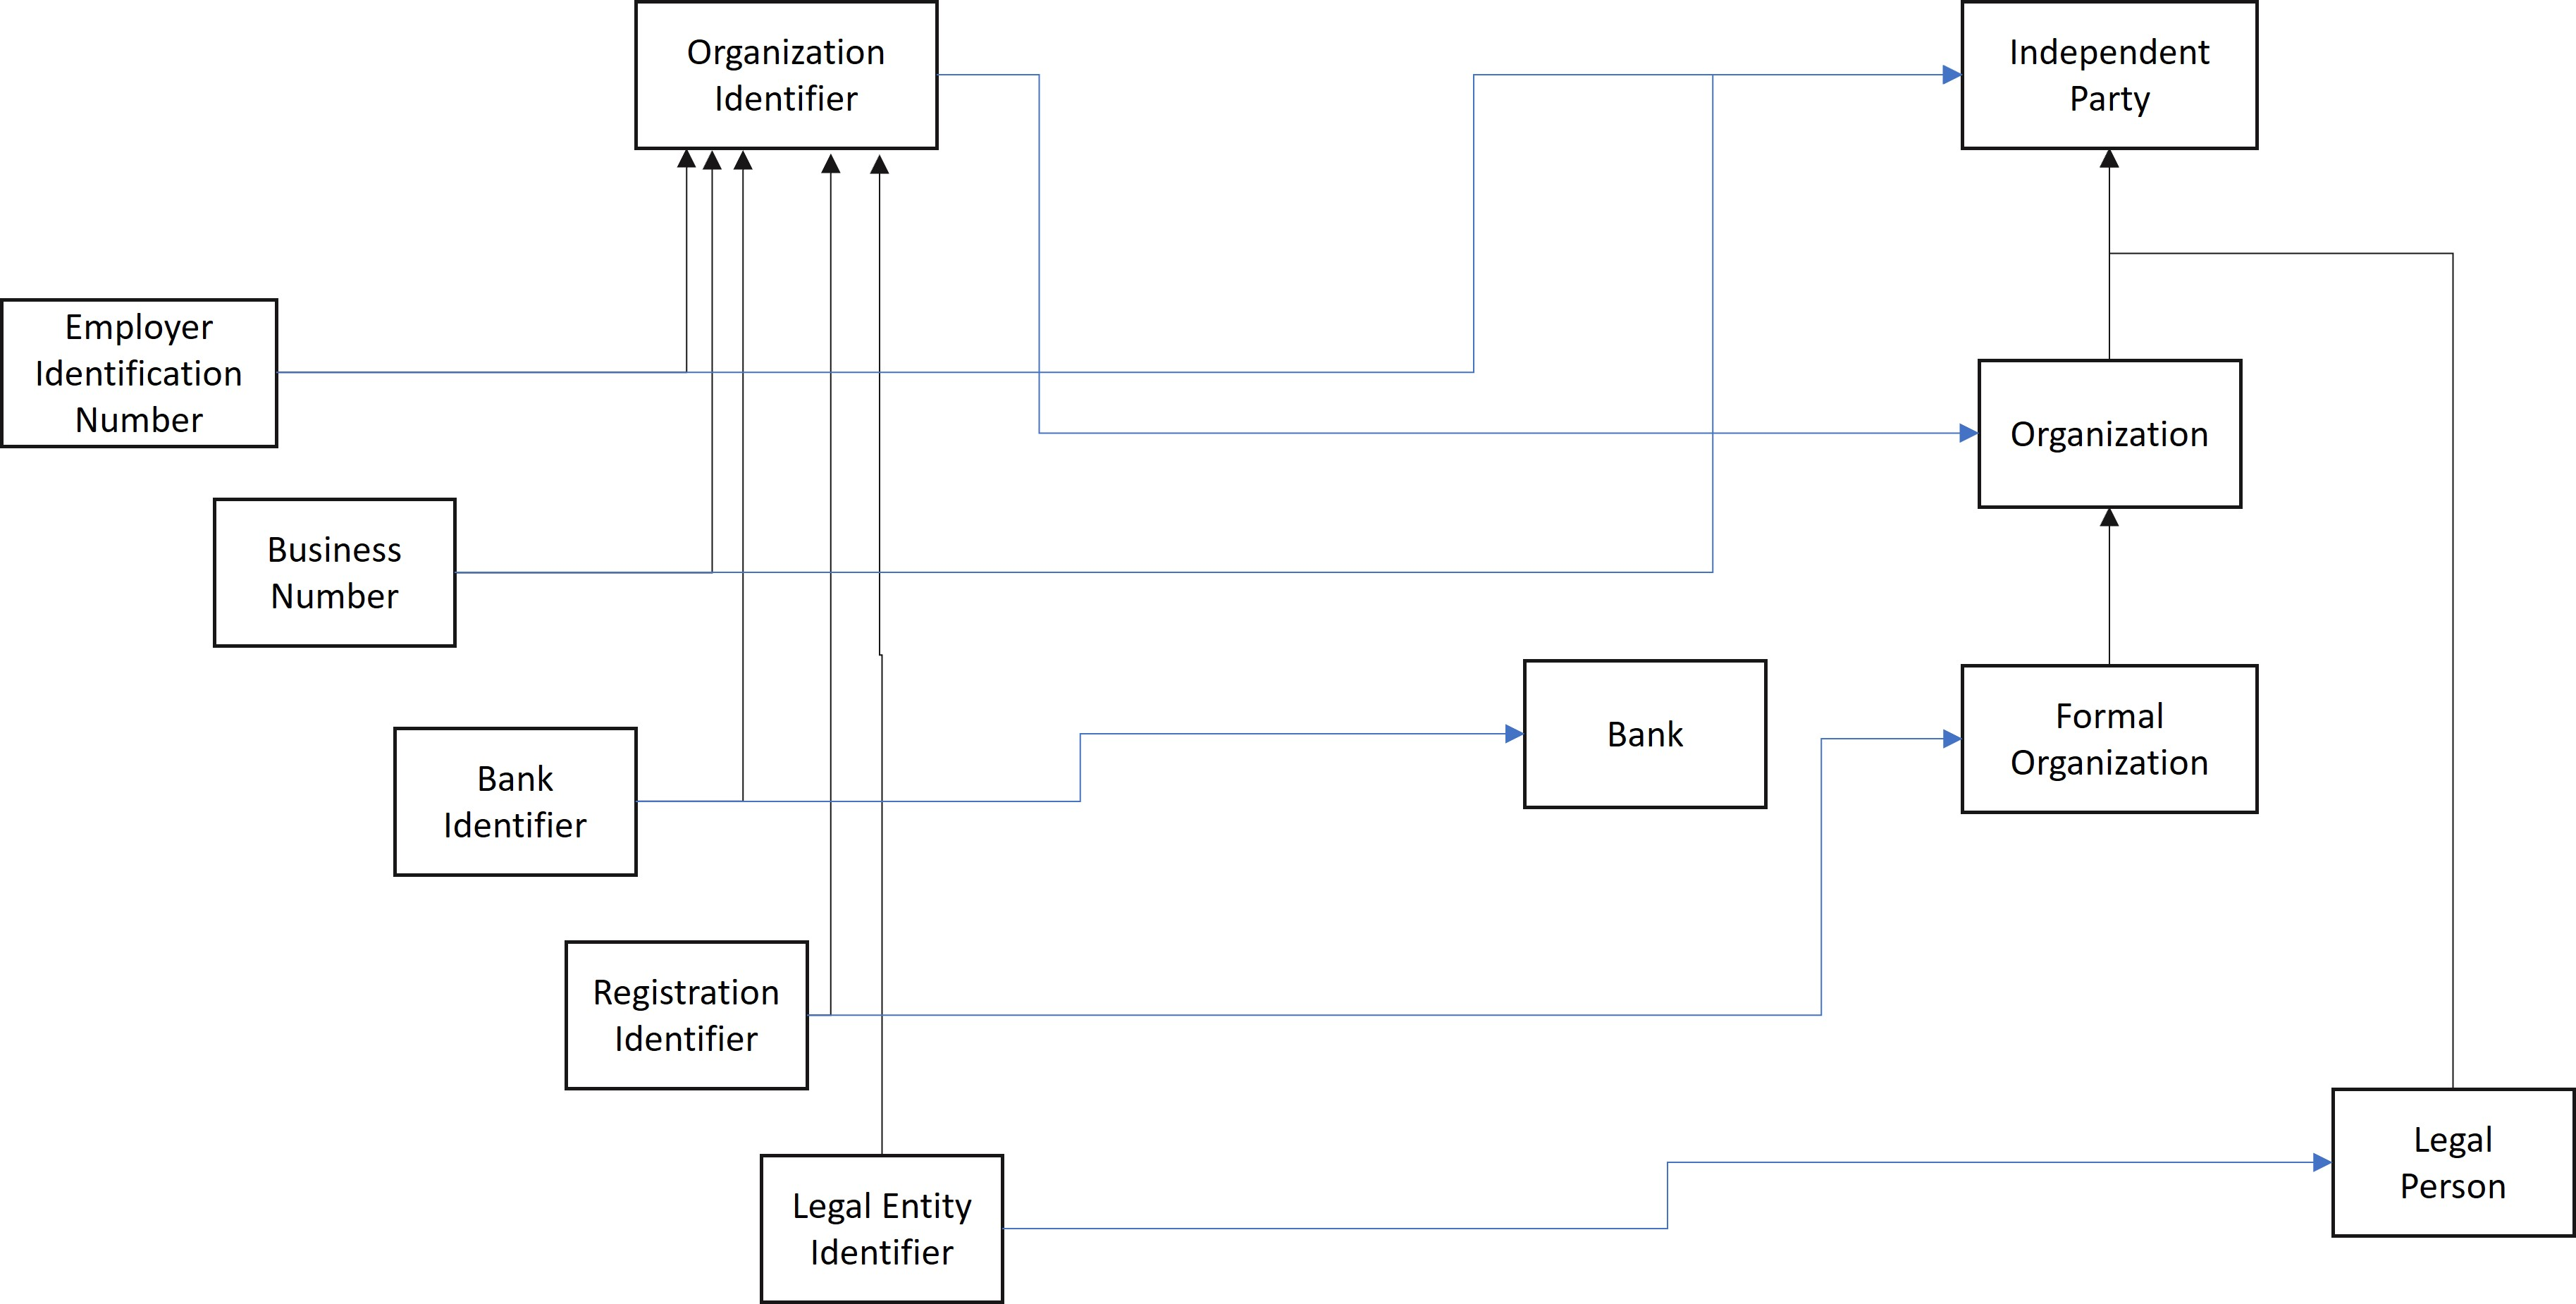
\includegraphics[width=3.3in]{figures/id-entity.jpg}
\caption{Representing identifiers as entities in their own right.  }
\label{ch01.fig4} 
\end{figure}

At an industrial level, FIBO has to be able to manage any number of identifiers, including the hundreds that appear at the enterprise level, and indeed, all of these identifiers for all enterprises.  This is where FIBO needs to anticipate the data structures in enterprises that it hasn't seen yet; will a new enterprise have an identifier that we haven't seen before?  Since we haven't seen that enterprise yet, we don't really know for sure, but it is a pretty good bet (given that the ones we have seen already have a hundred such identifiers!), that there will be new ones.  FIBO has to anticipate what it will see in these new enterprise data structures; the smart money says to expect there to be more identifiers thant we have heard of. 

For this reason, FIBO represents identifiers as shown in Figure \ref{ch01.fig5}, that is, as a separate data entity from the legal entity itself.  In addition, FIBO recognizes that many identifiers (like the SEC code and the LEI) have governing bodies that manage them, and that provide certain guarantees.  For example, a corporate EIN is issued by a particular state in the US, but is unique across all 50 states.  The LEI is managed by the Global LEI Foundation (GLEIF).  Some identifiers don't have a governing body.  It is useful, when comparing identifiers or understanding their scope, to know how they are governed.  For this reason, FIBO goes one step further, and represents not only the identifier, but also the identifier scheme, the registry that records the identifiers, and the jurisdiction that gives that registry its authority, as shown in Figure \ref{ch01.fig6}.






Build up an example of identifiers; an application can just have a number as an identifier.  An enterprise model will want to reify this, to take into account multiple id systems in the firm.  An industrial model will have to entertain the idea of kinds of id system providers; which ones do we recognize and which ones don't we? 




TEXT ENDS HERE


\section{Introduction}

Thus far in the book, the term \textit{information}
\index{information}%
has been used sparingly and when
it has been used, we have purposely been imprecise as to its meaning.



\begin{figure}[hbt] % 01
\centering
  \figboxes
\caption{Communication system block diagram.}
\label{ch01.fig2} 
\end{figure}

Examples of side-by-side figures.

%  F 2
\begin{figure}[hbt]%
\centering
\begin{subfigure}[t]{0.45\textwidth}%
	\smfigboxes
\caption{Annotated visualization of the structure of a biological neuron, reconstructed from electron microscope images of 30nm-thick slices of a mouse 
brain~\cite{tesniere59}.}%
\label{fig:bioneuron}%
\end{subfigure}%
\qquad%
\begin{subfigure}[t]{0.45\textwidth}%
	\smfigboxes
\caption{The shape of an action potential. A small external voltage stimulus (blue) triggers a cascade of charge build-up inside a neuron (red) via voltage-gated ion channels. The activation threshold is shown as a dotted line. Simulated using a Hodgkin-Huxley model of a neuron~\protect\cite{weber-97}.}%
\label{fig:ap}%
\end{subfigure}%
\caption{The structure and operation of biological neurons.}%
\end{figure}

%  F 3
\begin{figure}[b]
\centering
\begin{subfigure}[t]{0.45\textwidth}
	\smfigboxes
\caption{Points in $\mathbb{R}^2$, subdivided by a single linear classifier. One simple way of understanding linear classifiers is as a line (or hyper-plane, in higher dimensions) which splits space into two regions. In this example, points above the line are mapped to class 1 (red); those below, to class 0 (blue).}
\label{subfig:linclass}
\end{subfigure}%
\qquad%
\begin{subfigure}[t]{0.45\textwidth}
	\smfigboxes
\caption{Points in $\mathbb{R}^2$, subdivided by a combination of four linear classifiers. Each classifier maps \emph{all} points to class 0 or 1, and an additional linear classifier is used to combine the four. This hierarchical model is strictly more expressive than any linear classifier by itself.}
\label{subfig:circclass}
\end{subfigure}%
\caption{Simple elements can be combined to express more complex relationships.
This is one basic tenet of deep neural networks.}
\label{fig:classifiers}
\end{figure}


\section{Entropy and Average Mutual Information}
\label{ch01.sec2}

Consider a discrete random variable $U$ that takes on
the values $\{u_1, u_2, \dots, u_M\}$, where the set of possible
values of $U$ is often called the \textit{alphabet} and the elements
of the set are called \textit{letters} of the alphabet. Let $P_U(u)$
denote the probability  assignment  over the alphabet, then we can
define the \textit{self-information} of the event $ u = u_j $ by
\begin{equation}
  I_U \left( u_j \right) = \log \frac{1}{P_U (u_j)} = - \log P_U
    \left( u_j \right).
\label{ch01.eq1}
\end{equation}

\begin{example}
\label{ch01.ex1}
Given a random variable $U$ with four equally likely letters
in its alphabet, we wish to find $H(U)$. Clearly, $M=4$
and $P_U(u_i)= \tfrac{1}{4}$ for $ i = 1, 2, 3, 4 $.

\begin{align}
    I_{W;X}\left(w_j;x_k\right)
    & = \log
    \frac{P_{WX}\left(w_j, x_k\right)}{P_W\left(w_j\right)
              P_X\left(x_k\right)}
    \notag\\
    & = \log
    \frac{P_{X|W} \left( x_k | w_j\right)} {P_X \left(x_k\right)}
    =
     I_{X;W} \left(x_k; w_j\right).
\label{ch01.eq2}
\end{align}
\end{example}

\begin{property}
\label{ch01.pro1}
Let $U$ be a random variable with possible values $\{u_1,u_2,\dots, u_M\}$.
\end{property}

Example~\ref{ch01.ex1} illustrates Property~\ref{ch01.pro1}.

\begin{property}
\label{ch01.pro2}
Let $W$ and $X$ be jointly distributed random variables.
\end{property}

\begin{example}
\label{ch01.ex2}
Here we wish to calculate the mutual information and the average
mutual information for the probability assignments
(with $M=2$ and $N=2$)
\begin{equation}
 P_W \big(w_1\big) = P_W \big(w_2\big) = \tfrac{1}{2}
\label{ch01.eq3}
\end{equation}
\end{example}

\begin{example}[\cite{Boeringer}]
\label{ch01.ex3}
The source output is a ternary-valued random variable that takes on the
values $\{ u_1, u_2, u_3 \}$ with probabilities
$P(u_1) = 0.7, P(u_2) = 0.15 = P(u_3)$. 
\end{example}

\begin{theorem}[(Source Coding Theorem).]
\label{ch01.th1}
For a DMS with entropy $H(U)$,
the minimum average codeword length per source letter $(\bar{n})$ for any
code is lower
bounded by $H(U)$, that is, $\bar{n} \geq H(U)$, and further, $\bar{n}$
can be made as close to $H(U)$
as desired for some suitably chosen code.
\end{theorem}

\begin{theorem}[(Channel Coding Theorem~\cite{Wen-ChungLiu2005}).]
\label{ch01.th2}
Given a DMS
with entropy $H$ bits/source letter and a DMC with capacity $C$
bits/source letter,
if $H \leq C$, the source output can be encoded for transmission over
the channel with
an arbitrarily small bit error probability. Further, if $H > C$, the bit error
probability is bounded away from $0$.
\end{theorem}

\begin{proof}
This result can be proved in several ways, including calculus of
variations~\cite{WenWangetal2005} inequality; however, an
alternative method is used here.
\end{proof}

\begin{table}[hbt]
\caption{Timer0 Compare Output Mode, non-PWM Mode}
\label{ch01.tab1} 
\begin{center}
\begin{tabular}{|c|l|}
    \cb COM0x1-0
  & \cb Description 
\\
    \cw 00
  & \cw Normal port operation
\\
    \cy 01
  & \cy Toggle on Compare Match
\\
    \cw 10
  & \cw Clear on Compare Match
\\
    \cy 11
  & \cy Set on Compare Match
\\
\hline
\end{tabular}
\end{center}
\end{table}


\begin{center}
\begin{tabular}{|cl|}
    \cb COM0x1-0
  & \cb Description 
\\
    \cw 00
  & \cw Normal port operation
\\
    \cy 01
  & \cy Toggle on Compare Match
\\
    \cw 10
  & \cw Clear on Compare Match
\\
    \cy 11
  & \cy Set on Compare Match
\\
\hline
\end{tabular}
\end{center}


\section*{Summary}

In this chapter we have discussed very briefly some of the salient
results from information theory and rate distortion theory and have
indicated how these results can be used to bound communication system
performance.


\section*{Problems}
\index{problems}%

\begin{problems}

\item
A random variable $U$ has a sample space consisting of the set
of all possible binary sequences of length $N$, denoted
$\{u_j, j=1, 2, \ldots, 2^N \}$.

\item
Given a random variable $U$ with the alphabet $\{ u_1, u_2, u_3, u_4 \}$
and probability assignments $P(u_1) = 0.8, P(u_2)=0.1$,
$P(u_3) = 0.05, P(u_4)=0.05$, calculate the entropy of $U$.
Compare your result to a random variable with equally likely values.

\end{problems}

\clearpage

